\documentclass[0-thesis.tex]{subfiles}

\begin{document}
\label{chap:profiles}
The previous two sections have proposed a technology agnostic update architecture and a
life cycle perspective for devices. It is time to show concrete incarnations of this
architecture using state of the art IoT protocols. This section is aimed towards
implementers needing to make decisions about how to implement the update architecture.
This section will discuss choice of image digest algorithm, vendor and class ID
generation, payload encoding and encryption, and considerations when choosing between
DTLS/CoAP and OSCORE for an update architecture profile.

\subsection{DTLS Profile}
\label{sec:dtls-profile}
When implementing the architecture, one choice of protocols is using DTLS and CoAP for
constrained communication to and from devices. For enrollment and authorization, EST and
ACE can be used with their respective suitable profiles. However, as DTLS provides
security at the transport layer it cannot be used for broadcasting, \gls{oscore} is an
option better suited for broadcasting. 

DTLS is already profiled for use in IoT contexts and EST and ACE profiles are works in
progress \parencite{rfc7925, est-coaps, ace-dtls-profile}. The update architecture needs
little extra profiling in addition to these protocols, namely image digest algorithm,
vendor and class ID generation, payload encoding, and payload encryption. The security of
the architecture is not bound to characteristics of any of these protocols and others can
be used instead, this is just one possible profile.

\begin{figure}
    \caption{The various protocols used in the DTLS profile. Protocols outside the constrained networks are suggestions.}
    \label{fig:dtls-profile}
    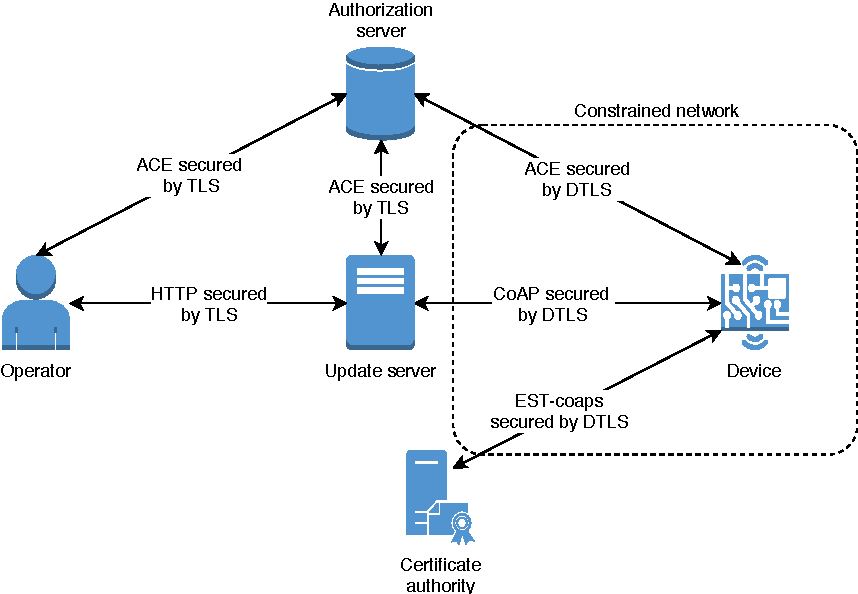
\includegraphics{images/dtls-profile.pdf}
\end{figure}

\subsection{ID Generation and Hash Algorithms}
\label{ssec:hash-id-algorithm}
The DTLS IoT profile suggests ciphersuites for the use of pre-shared keys and certificates
and EST has been profiled with CoAPs to use the same ciphersuites for certificates. These
suites implement the \textbf{SHA-256} hash function which can be used to calculate the
digest of an image. Since the digest is just supposed to verify the integrity of the
image, SHA-256 is an adequate choice and does not require implementing new hash algorithms
for devices already running DTLS.

Generating vendor and class IDs should be done so that devices get unique identifiers and
devices with the same names from different vendors do not clash. For this purpose,
\textbf{UUIDs} can be used \parencite{rfc4122}. Version 3 and 5 of UUID are "name-based"
versions meaning they operate in a given namespace. By using a registered domain name of
the vendor, which is already guaranteed to be unique, as namespace a unique UUID can be
generated for that vendor. By using the vendor UUID as the namespace for the class IDs,
devices from different vendors can share names but still have different class IDs. A
hierarchical namespace structure is suggested also by SUIT.

Section 4.3 of the UUID specification states that "Choose either MD5 or SHA-1 as the hash
algorithm; If backward compatibility is not an issue, SHA-1 is preferred". This means
\textbf{UUID5} should be used as it uses SHA-1 for hashing. ID generation will not occur on the
devices themselves, devices only need to be prepared with their IDs for comparing with the
manifest.

\subsection{Payload Encoding and Encryption}
\label{ssec:encoding-encryption}
For encoding, \textbf{\gls{cbor}} is an efficient binary encoding \parencite{rfc7049}.
CBOR aims to be an extensible data format providing very small code sizes. It supports
simple values as well as arrays and maps meaning it is easy to map to and from JSON while
being more compact than JSON. 

The use of CBOR enables the use of \textbf{\gls{cose}}. COSE provides encryption and signing for
CBOR encoded objects, which in the architecture will be the manifest and image
\parencite{rfc8152}. As DTLS secures the channel, the manifest and image can be signed
using COSE objects to ensure their integrity during transport. 

\subsection{OSCORE Profile}
\label{sec:oscore-profile}
The main difference between using CoAP over DTLS and OSCORE is on which level the
communication is secured. DTLS provides transport layer security by setting up a secure
channel for communication. This means payloads are encrypted but the secure channel ends
at for instance a proxy or update server. DTLS does not provide end-to-end security and as
the security provided is on a transport level it is not compatible with broadcasting. The
architecture itself does not impose restrictions towards broadcasting updates, but a
profile based on the security granted by DTLS will not support it. In order to support
broadcasting, OSCORE can be used instead.

OSCORE provides end-to-end protection for CoAP messages using COSE \parencite{oscore}. By
providing end-to-end encryption CoAP message security is not terminated at a proxy or
update server as with DTLS. This means a compromised proxy or update server cannot be
leveraged to eavesdrop or manipulate data. The difference between using OSCORE and using
COSE payloads in CoAP with DTLS is that OSCORE protects the entire CoAP message end-to-end
while COSE and CoAP protects only the payloads but not the CoAP message itself, it relies
on a secure channel established by DTLS. 
% TODO: Add part about operator pushing manifest to device and having it protected

\begin{figure}
    \caption{The various protocols used in the OSCORE profile. Protocols outside the constrained networks are suggestions.}
    \label{fig:oscore-profile}
    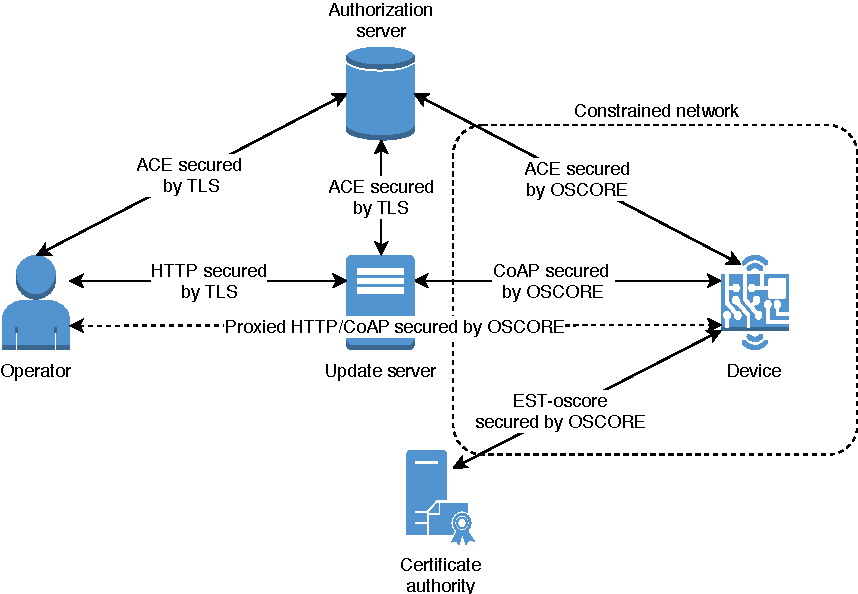
\includegraphics{images/oscore-profile.pdf}
\end{figure}

OSCORE can run directly on top of UDP and supports broadcasting as well as unicast. In the
case of broadcasting, a security context must be defined \parencite{oscore-group}. If a
security context is in place, unicast OSCORE is still possible. At the time of writing,
there are two Internet-Drafts aiming to specify profiles for ACE and EST using OSCORE,
meaning these protocols can be used for enrollment and authorization with OSCORE as well
\parencite{ace-oscore, est-oscore}. ID generation, hash algorithms, and payload encoding
and signing in the OSCORE profile is the same as in the DTLS profile, see section
\ref{ssec:hash-id-algorithm} and \ref{ssec:encoding-encryption}.

Broadcasting is of interest in the update architecture as communication between update
servers and devices can be one-to-one, many-to-one, one-to-many, or many-to-many. It is
dependant on the topology of the network and how update servers are mapped to devices and
thus logically dividing the network. In order to efficiently update many devices of the
same class or from the same vendor, broadcasting can be employed. The information in the
manifest makes sure that devices receiving broadcasted updates not intended for them does
not erroneously install the update.

While being better suited for broadcasting and providing end-to-end security, OSCORE is
not yet standardized. The specification (\parencite{oscore}) is a work in progress as is
many of the profiles mentioned in this section. DTLS and its related IoT profiles are
standardized and much more mature. If implementing the architecture using OSCORE, it is
worth noting the incomplete status of the standard.

\subsection{Summary}
\label{sec:5-summary}
This section identified two options for implementing the architecture: either CoAP over
DTLS or OSCORE. TLS does not support broadcasting however which might be of importance,
for this purpose OSCORE can be used instead. OSCORE does not rely on a secure channel
established by DTLS but instead provides end-to-end security for CoAP messages using COSE.
OSCORE, unlike DTLS, is not yet standardized and the author is not aware of any OSCORE
implementation in Contiki-NG. 

Both approaches would use SHA-256 for calculating image digests, UUID5 for vendor and
class IDs using registered vendor domains, EST with its corresponding profile for
enrollment, and ACE with its corresponding profile for authorization. Payloads are encoded
and signed using CBOR and COSE for both approaches, ensuring integrity.

With the proposed profiles, a prototype can be implemented and evaluated. Implementation
of the prototype is the topic of the next chapter.

\end{document}